\documentclass{article}
%\documentclass{amsart}
%\documentclass{letter}

\usepackage{a4}
%\addtolength{\evensidemargin}{-1.5cm}
%\addtolength{\oddsidemargin}{-1.5cm}
%\addtolength{\textwidth}{3cm}
%\addtolength{\topmargin}{-2cm}
%\addtolength{\textheight}{2cm}

%|usepackage[english, hebrew]{babel}
%\sethebrew

\usepackage{amsmath, amssymb, amsthm}
\usepackage{graphicx}
\usepackage{subfigure}

\newtheorem*{proposition}{Proposition}
\newtheorem*{prop}{Proposition}
\newtheorem*{thm}{Theorem}
\newtheorem*{lem}{Lemma}
\newtheorem*{cor}{Corollary}
\newtheorem*{axiom}{Axiom}

\theoremstyle{definition}
\newtheorem*{define}{Definition}

\theoremstyle{remark}
\newtheorem*{remark}{Remark}

\setcounter{secnumdepth}{0}

%\newcommand{\qed}{\hfill $\Box$ \hfill \\}
%\newenvironment{proof}[1][Proof]
%{ \begin{itshape} \begin{trivlist}
%	\item[\hskip \labelsep \textbf{\textnormal{#1}}]}
%{ \end{trivlist} \end{itshape} }

\def \norm [#1]{\left\| #1 \right\|}

\title{Research Proposal}
\author{Hila Sheftel}
\date{30/9/2010}
\begin{document}

\begin{abstract}
We propose a model for multiple-objectives evolution in which several archetypes exist, 
each optimal for a certain objective or fitness function. 
These fitness functions define a set of optimal points on the space of possible species. In the suggested research – we propose to theoretically analyze the above model, and attempt to validate it by analysis of various data sets.
\end{abstract}
%\pagebreak
\section{Introduction}
The basic assumption of evolution is “survival of the fitted” - 
random mutations constantly occur, and there is a natural selection of those  mutations that are fittest in their environments. 
In the context of “multiple objective evolution”, 
the fitness is measured with respect to several “tasks” – e.g. - swimming, running etc. 
The evolutionary point of view dictates in that case that if organism $A$ is fitter than organism $B$ in every aspect 
(runs faster, swims better), organism $B$ will have less reproductive success. 
Each organism can be described by a collection of quantitative attributes 
(for example – length of feet, width of body and so forth). 
We consider a finite set of $n$ attributes. In that case, each organism can be represented as a vector in $\mathbb{R}^n$.
\section{Background}
Our research assumption is that there are $k$ “archetypes”: $x_1,\ldots,x_k \in \mathbb{R}^n$. 
Each archetype represents an organism that is optimal for dealing with a certain task that supports survival 
(e.g. - “the perfect swimmer” and “the perfect runner”). 
Denote by $X$ the subset of $\mathbb{R}^n$ that represent all of the observable organisms. 
For each $1\leq i \leq k$, there is a function $f_i: X \rightarrow \mathbb{R}$ 
which describes the fitness of an organism $x \in X$ to deal with the task $i$ . 
We assume that $f_i$ is maximal at the point $x_i$.
In this setting it is natural to define a partial order on $X$ as follows: 
For $y,z \in X$ we say that $y \succ z$ if for every $1\leq i \leq k$ $f_i(y)\geq f_i(z)$ 
and there exists $1\leq j \leq k$ such that $f_j(y) > f_j(z)$. 
The biological interpretation of this is that organism $y$ performs each task at least as well as organism $z$ 
and is strictly better in at least one of the tasks. 
\begin{define}
The \textit{Pareto Frontier} is the set of all maximal points in X with respect to this order.
\end{define}
The Pareto frontier consists of all organisms for which there doesn’t exist an organism that deals with every task better than them. 
Hence, it consists of all evolutionarily possible organisms. 

Within this framework, there are two open research directions which are of interest to me:
\begin{itemize} 
\item Analytically describing how the Pareto Frontier depends on various factors, such as the nature of the fitness functions $f_i$, 
the dimensionality of the attributes space,  the number of archetypes and so forth..
\item Examining the validity of the Pareto Frontier concept for describing different experimental data sets (specific phenotypes in various species). 
For each such data set - attempting to recover the archetypes and understand their biological nature.
\end{itemize}

So far, the first question has been answered in the following setting: 
Let $X = \mathbb{R}^n$. Assume an arbitrary inner product on $\mathbb{R}^n$. 
Denote the norm derived from this inner product by $\norm[.]$. 
Assume that all $f_i(x) = f_i(\norm[(x-xi)]$ and are strictly monotonically decreasing. 
In this setting, Dr Guy Shinar has proven that the Pareto Frontier $x_1,\ldots,x_k$ equals their convex hull.

As for the second research direction, some basic work was done on several data sets. For example:
\begin{itemize}
\item The sizes of molars of 29 murine rodents species were measured \cite{Teeth}. 
Denote the sizes of the 1st, 2nd and 3rd molars by $M_1$,$M_2$ and $M_3$ respectively. 
We place all rodents on a plane whose axes are $M_2/M_1$ and $M_3/M_1$ 
(see Figure 4c in \cite{Teeth}). 
It is shown that all existing rodents fall on a straight line between two points, 
or differently phrased, on the convex hull of these points. 
These results fit the model if the above mentioned points are taken to be the archetypes, 
and the fitness of each rodent to the archetype’s associated task is taken to simply be the distance 
in the $M_3/M_1 \times M_2/M_1$ plane. 
Under these assumptions, according to the above theorem the Pareto Frontier is the convex hull of the two archetypes. 
All that remains to be explained is which tasks the archetypes are designed to deal with. 
The first archetype's coordinates - $(1,1)$ correspond to a rodent whose all 3 molars are of the same size. 
The species plotted near this point are herbivorous. 
Hence, there is a reason to suspect that those proportions are anatomically suited for eating herbs. 
The second archetype's coordinates - $(0.55,0)$ 
correspond to a rodent whose first molar is twice the size of its second molar, 
and its 3rd molar is inexistent. 
The species that are plotted near this point are faunivorous. 
Hence, there is a reason to suspect that those proportions are anatomically suited for eating meat.
\item The lengths of the phalanges of approx. 70 bird species whose 4th digit has 4 phalanges were measured (see Figure \ref{fig:bones}). 
Denote the lengths of the 1st, 2nd, 3rd and 4th phalanges by    
$A_1,A_2,A_3$ and $A_4$ respectively. 
The data is placed on a three dimensional space whose axes are 
$A_2/A_1$, $A_3/A_1$ and $A_4/A_1$. 
The surprising phenomena is that most of the data lies on a plane.
Looking only at this plane, and discarding the raptors, all other points seem to form a triangle  (see Figure \ref{fig:birds}). 
A simple algorithm that searches for the smallest triangle that contains as many points as possible 
was applied on the data. 
The corners of the resulting triangle represent the 3 suspected archetypes. 
The first archetype corresponds to a bird whose 4 phalanges are of the same length. We suspect those 
proportions are optimal for grabbing. 
The second archetype corresponds to a bird whose first phalanx is very long. We 
suspect this is anatomically ideal for walking. 
The third archetype corresponds to a bird whose fourth phalanx is very long. We 
suspect this is anatomically ideal for digging. 
It is important to mention that those are just preliminary results, and further work is needed in order to 
properly establish the above claims.
\end{itemize}

\section{Proposed Research Goals}
As stated above – I would like to conduct research in two directions:
\begin{itemize}
  \item Approach the problem of theoretically describing the Pareto Frontier under different assumptions.
  \item Check the validity of the model according to which species are at the Pareto Frontier 
        of a number of archetypes, 
        by acquiring data for different species and attempting to recover the underlying archetypes.
\end{itemize}
The first step will be to approach the question of the Pareto Frontier’s shape 
for a more general case than the one already proven. 
In that case, the fitness functions are still of the form 
$f_i(x) = f_i(\norm[x-x_i])$. However, the used norm ($\norm[.]$) can be different for each archetype. 
This means that differing from one archetype doesn’t have the same biological implications as differing 
from a second archetype. The steps toward answering this question will be to:
\begin{itemize}
  \item Solve several examples numerically
  \item Use the obtained insights to phrase a hypothesis. 
  \item Prove it rigorously.
\end{itemize}

From this I hope to gain insight on how data that fit the model might look. 
I expect to discover that in the more general case the Pareto Frontier can differ from the convex hull.

The second step will be to build a data pool of relevant cases, 
such as length of birds fingers , shape of dogs teeth, colour of butterflies wings and so forth, and check if they fit the model.
Doing this will require to deal with the following tasks:
\begin{itemize}
  \item Develop a statistical framework for determining how well a data set supports our model. 
	How can one statistically differentiate between random data and data that forms a Pareto Frontier? 
	One possible sign is if the data has a lower dimensionality than that of the attributes space. 
	Are there other tests?
  \item Think of a statistical test to check if the data is a convex hull of a finite set of points. 
	This question becomes more complicated if we also consider the possibility that some of the 
	archetypes themselves are not existent in nature. 
	This might form a convex hull with regions that aren't occupied by any existent species. 
	Develop an algorithm to best determine the number and locations of archetypes.
  \item Try to infer the biological functions of the various archetypes from the data.
\end{itemize}



More questions to approach:
Is there a biological mechanism that guarantees that the evolution will be performed only on the Pareto Frontier?
Can this principle (species reside in the Pareto Frontier generated by a number of archetypes) 
be generalized to describe other phenomena in nature, such as enzymes design?

\pagebreak

\begin{figure}
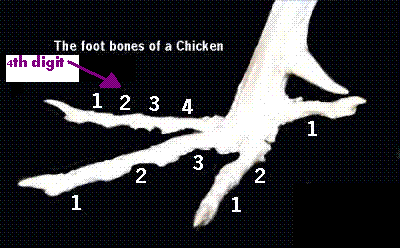
\includegraphics[width=0.4in]{bones.png}
\caption{A bird whose 4th digit has four phalanges.}

\label{fig:bones}
\end{figure}

\begin{figure}
\centering
\subfigure[]{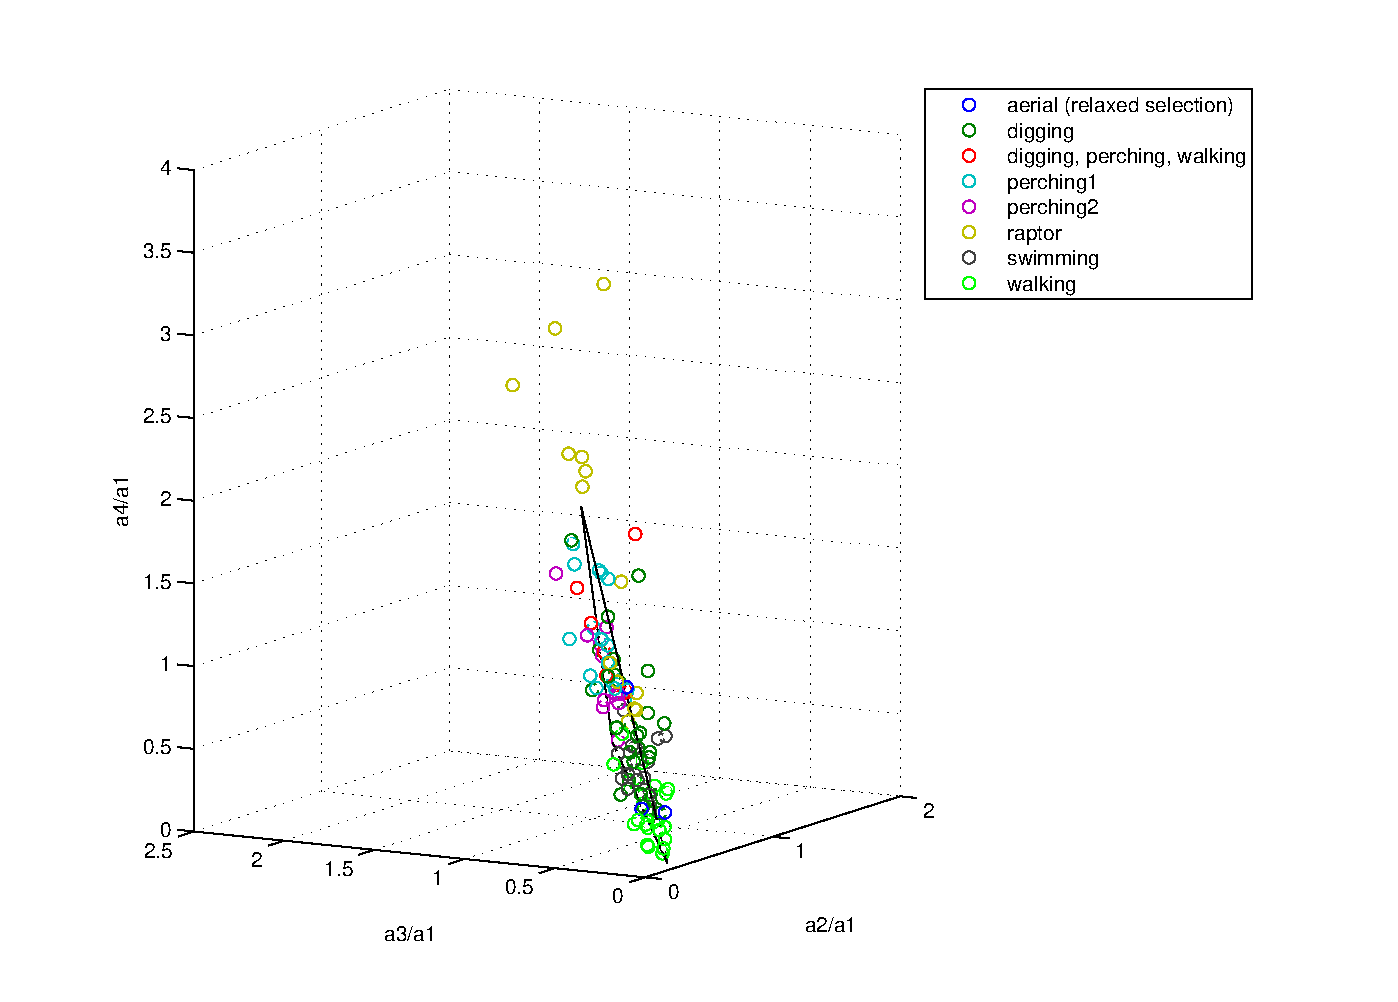
\includegraphics[width=2.4in]{birds2.eps}}
\subfigure[]{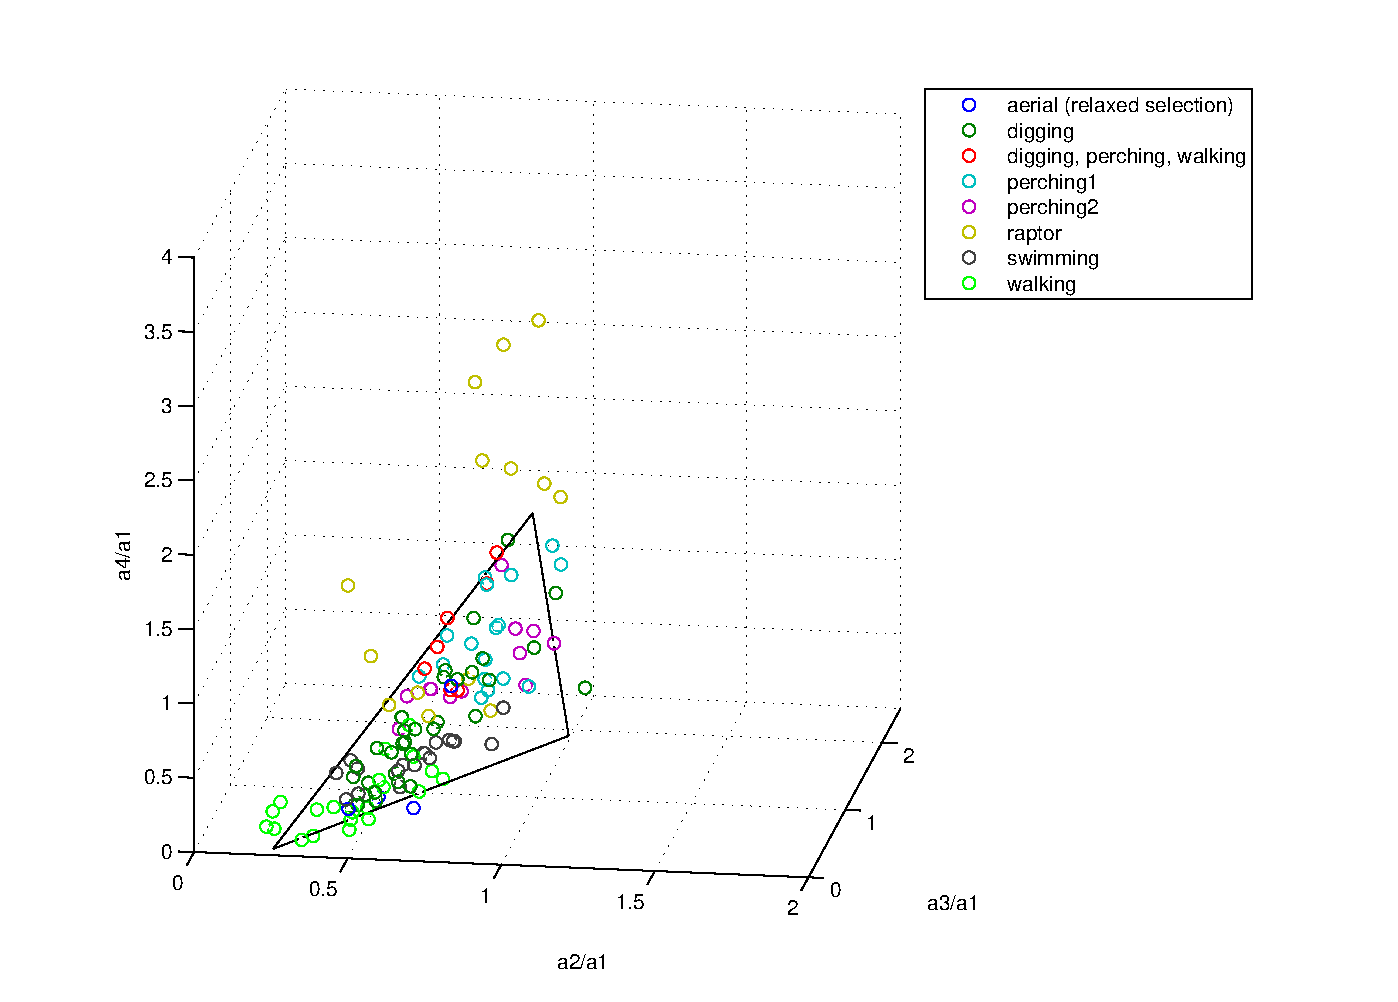
\includegraphics[width=2.4in]{birds1.eps}}
\caption{Each circle represent a bird species. $a_1, a_2, a_3$ and $a_4$ are the lengths of the 1st, 2nd, 3rd and 4th phalanx of that species' 4th digit, respectively. The colour of the circle represents the species' functional family. It can be seen that most of the data lies on a plane (a). Looking at this plane, and discarding the raptors, the data circles seem to form a triangle (b). The approximated triangle is plotted on the figure (black solid line).} 

\label{fig:birds}
\end{figure}

\bibliographystyle{plain}
\bibliography{proposal}

\end{document}
 

 
